\documentclass[tikz,border=2pt]{standalone}
\usepackage{amsmath,amssymb}
\usepackage{tikz}

\begin{document}
% Any intersection of closed sets is closed; a finite union is closed; an infinite union need
% not be: the closed intervals [1/n, 1] pile up to (0, 1], which is not closed.
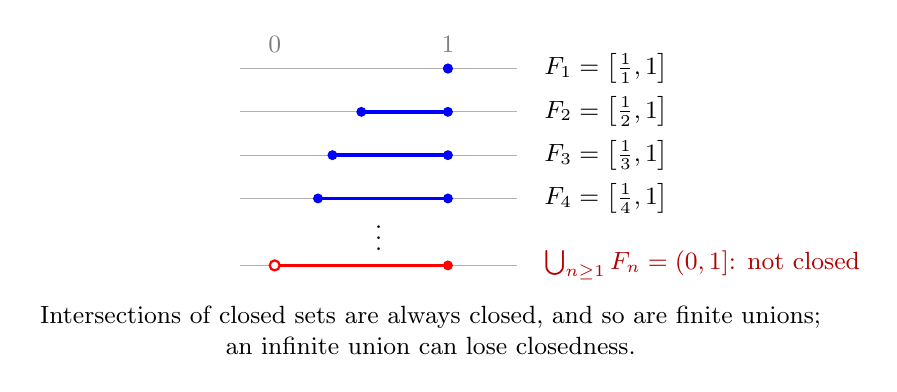
\begin{tikzpicture}[x=2.2cm, every node/.style={font=\small}]
	\node[font=\small, gray] at (0,0.3) {$0$};
	\node[font=\small, gray] at (1,0.3) {$1$};
	\foreach \n/\y in {1/0, 2/-0.55, 3/-1.1, 4/-1.65} {
		\draw[gray!60] (-0.2,\y) -- (1.4,\y);
		\draw[very thick, blue] ({1/\n},\y) -- (1,\y);
		\fill[blue] ({1/\n},\y) circle (1.8pt);
		\fill[blue] (1,\y) circle (1.8pt);
		\node[anchor=west] at (1.5,\y) {$F_{\n}=\left[\tfrac1{\n},1\right]$};
	}
	\node at (0.6,-2.05) {$\vdots$};
	\draw[gray!60] (-0.2,-2.5) -- (1.4,-2.5);
	\draw[very thick, red] (0,-2.5) -- (1,-2.5);
	\draw[red, thick, fill=white] (0,-2.5) circle (1.8pt);
	\fill[red] (1,-2.5) circle (1.8pt);
	\node[anchor=west, red!70!black] at (1.5,-2.5) {$\bigcup_{n\ge1}F_n=(0,1]$: not closed};
	\node[anchor=north, align=flush center, text width=10cm] at (0.9,-2.9) {Intersections of closed sets are always closed, and so are finite unions; an infinite union can lose closedness.};
\end{tikzpicture}
\end{document}
